\documentclass[../kl10.tex]{subfiles}
\graphicspath{{\subfix{../images/}}}



\renewcommand{\arraystretch}{1.2}
\begin{document}

\section{Gase sind meine Phase}
Die kinetische Gastheorie ist ein Teilgebiet der statistischen Mechanik. Mithilfe der kinetischen Gastheorie sind thermodynamische und kinetische Verhaltensweisen von Gasen anschaulich auf molekularer Ebene erklärbar. Die kinetische Gastheorie verwendet dabei die Modellvorstellung des idealen Gases.
\enumaufgabe{\operator{Kreuze an}, welche der folgenden Grundannahmen nach dem Modell des idealen Gases getroffen werden.}

\begin{tabularx}{\textwidth}{|X|C{1.5cm}|C{1.5cm}|}\hline
    Nach den Modellannahmen des idealen Gases… & wahr & falsch\\\hline
    …ist das Eigenvolumen von Gasteilchen vernachlässigbar klein gegenüber dem \ \  Systemvolumen. & \solutiontext{\checkedbox}{\emptybox} & \emptybox \\\hline
    …haben die Gasteilchen ein nicht zu vernachlässigendes Volumen, sind aber alle \ \ \ \ kugelförmig.& \emptybox  & \solutiontext{\checkedbox}{\emptybox}  \\\hline
    …werden die Gasteilchen als Würfel genähert.& \emptybox & \solutiontext{\checkedbox}{\emptybox} \\\hline
    …wirken zwischen den Gasteilchen lediglich anziehende Wechselwirkungen.& \emptybox & \solutiontext{\checkedbox}{\emptybox} \\\hline
    …gibt es zwischen den Gasteilchen keine anziehenden und abstoßenden Kräfte. \ \ \ \ Die Teilchen können lediglich ideal elastisch miteinander stoßen. & \solutiontext{\checkedbox}{\emptybox} & \emptybox \\\hline
    …besitzen die Teilchen lediglich Rotationsenergie, aber keine kinetische Energie. & \emptybox & \solutiontext{\checkedbox}{\emptybox} \\\hline
    …besitzen die Teilchen lediglich Vibrationsenergie, aber keine Rotationsenergie. \ \ \ Über die kinetische Energie wird keine Aussage getroffen.& \emptybox & \solutiontext{\checkedbox}{\emptybox} \\\hline
    …besitzen die Teilchen keine potentielle Energie. & \solutiontext{\checkedbox}{\emptybox} & \emptybox \\\hline
    
\end{tabularx}
\solutiontext{je richtiges Kreuz 0,5P, je falschem Kreuz -0,5P => max 4P., nicht weniger als 0P
}{0.5cm}

Nach der kinetischen Gastheorie besitzen nicht alle Gasteilchen eines Gases die gleiche Geschwindigkeit. Die Geschwindigkeitsverteilung ergibt sich jedoch aus der sogenannten \textsc{Maxwell-Boltzmann}-Verteilung. Die \textsc{Maxwell-Boltzmann}-Verteilung für Argon bei einer Temperatur von 298\thinspace K ist im Folgenden dargestellt:

\begin{figure}[H]
    \centering
    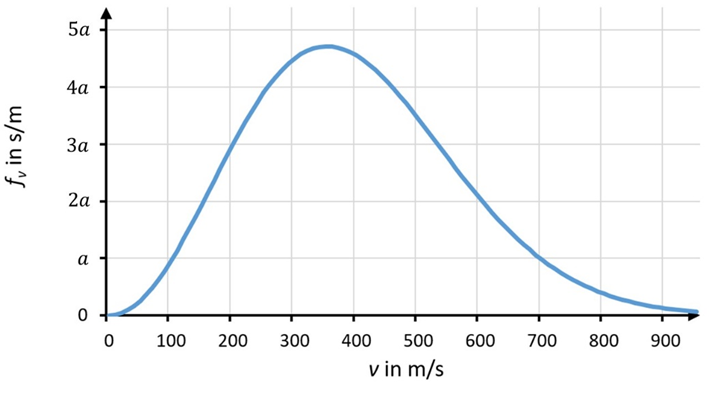
\includegraphics[width=0.7\textwidth]{2024/Abbildungen/Kinetisch_Gas/M-B-Verteilung.png}
\end{figure}

Auf der x-Achse ist dabei die Geschwindigkeit $v$ dargestellt und auf der y-Achse der Wert der Funktion $f_v$, welche die Geschwindigkeitsverteilung der Teilchen beschreibt. Ein größerer Wert bedeutet dabei, dass mehr Teilchen diese Geschwindigkeit besitzen. Beachte, dass die y-Achse im obigen Diagramm noch nicht skaliert ist. Die Variable $a$ ist dabei eine positive reelle Zahl. 
Die Wahrscheinlichkeit $p$ ein zufällig ausgewähltes Teilchen anzutreffen, welches eine Geschwindigkeit zwischen $v_1$ und $v_2$ besitzt, lässt sich näherungsweise berechnen durch:
$p\approx f_{v_1}\cdot (v_2-v_1)$.
Die Differenz zwischen $v_2$ und $v_1$ muss dabei gering sein, sodass gilt: $f_{v_1} \approx f_{v_2}$.

\newpage

\enumaufgabe{\operator{Gib} näherungsweise die Geschwindigkeit \operator{an}, welche ein zufällig ausgewähltes Argon-Atom bei $\SI{298}{\kelvin}$ am wahrscheinlichsten besitzt.}

\solution{Ca. $\SI{350}{\meter\per\second}$ (1P, alles im Bereich von $\SI{330}{\meter\per\second}$ bis $\SI{370}{\meter\per\second}$ als korrekt zu werten)\\
Insg. 1P
}{2cm}

\enumaufgabe{\operator{Begründe} kurz, ob die durchschnittliche Geschwindigkeit der Argon-Atome identisch mit der in Teilaufgabe b) bestimmten wahrscheinlichsten Geschwindigkeit ist. Wenn nein, \operator{gib an}, welche der beiden Geschwindigkeiten größer ist.}

\solution{Nicht identisch (1P), da die \textsc{Maxwell-Boltzmann}-Verteilung unsymmetrisch ist. (äquivalente Erklärungen möglich) (1P)\\
Die durchschnittliche Geschwindigkeit ist größer als die wahrscheinlichste Geschwindigkeit. (1P)\\
Insg. 3 P.
}{4cm}

\enumaufgabe{\operator{Begründe} kurz, welchen Wert die Fläche besitzt, welche zwischen dem Graphen $f_v$ und der x-Achse eingeschlossen wird. (Mathematisch formuliert: Welchen Wert besitzt das Integral $\int_0^{\infty} f_v \mathrm{d}v$?)}

\solution{1 (1 P.) \\
Die Wahrscheinlichkeit, dass ein Teilchen eine Geschwindigkeit zwischen 0 und unendlich besitzt muss 100\thinspace \% sein. Alternativ: negative Geschwindigkeiten sind nicht physikalisch sinnvoll. (weitere äquivalente Erklärungen möglich) (1P)\\
Insg. 2P
}{4cm}

\newpage

\enumaufgabe{\operator{Ermittle} den Zahlenwert für $a$. \operator{Führe} dazu eine graphische Integration („Kästchen zählen“) in dem Diagramm auf dem Antwortbogen \operator{durch}.}

\solution{
\begin{figure}[H]
    \centering
    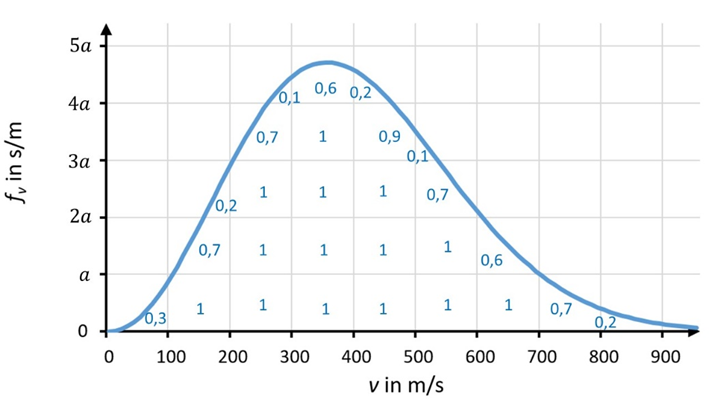
\includegraphics[width=0.7\textwidth]{2024/Abbildungen/Kinetisch_Gas/MB_Verteilung_Lsg.png}
\end{figure}
1,5 P., wenn erkennbar, dass Kästchen gezählt wurden (auch geben, wenn korrekte Anzahl Kästchen angegeben, aber kein Zählen explizit erkennbar)\\
Gezählte Kästchen: 20 (1,5 P.) (alles im Bereich 17 bis 23 Kästchen als korrekt zu werten).\\
$$1=20\cdot(a \thinspace\mathrm{s/m} \cdot 100 \thinspace\mathrm{m/s})$$ (2 P. für Ansatz) \\
$$a=\frac{1}{20\cdot100}$$
$$a=0,0005$$ (1P auf Ergebnis) \\
Insg. 6P
}{13cm}

\enumaufgabe{\operator{Berechne} näherungsweise den Anteil an Argon-Atomen, welche bei \SI{298}{\kelvin} eine Geschwindigkeit zwischen \SI{200}{\meter\per\second} und \SI{205}{\meter\per\second} besitzen. \\Solltest du Teilaufgabe e) nicht gelöst haben, so nimm $a=0,001$ an.}

\solution{
$$f_{200 \thinspace \mathrm{m/s}}\approx 3a\cdot\thinspace \mathrm{s/m}=0,0015\thinspace \mathrm{s/m}$$   (1P auf Abslesen, alles im Bereich von 2,8a  s/m bis 3,2a  s/m als korrekt zu werten)\\
$$p\approx f_{200 \thinspace \mathrm{m/s}} \cdot (v_2-v_1 )=0,015  \thinspace \mathrm{s/m} \cdot (205 \thinspace \mathrm{m/s}-200 \thinspace \mathrm{m/s})$$ (0,5 P. auf Ansatz)\\
$$p\approx 0,0075=0,75\%$$ (0,5 P. auf Ergebnis, alles zwischen 0,7\% und 0,8\% als korrekt zu werten) \ \ \ Insg. 2P \\ 
Ergebnis mit Ersatzannahme: $f_{200 \thinspace \mathrm{m/s}}\approx 0,003\thinspace \mathrm{s/m}$; $p\approx 0,015=1,5\%$ (alles zwischen 1,4\% und 1,5\% als korrekt zu werten)\\
}{5.5cm}

Die Geschwindigkeitsverteilung von Gasteilchen ist nach der \textsc{Maxwell-Boltzmann}-Verteilung abhängig von Temperatur und Teilchenmasse. Die Wahrscheinlichkeit $p_{v<v_{max}}$ ein zufällig ausgewähltes Teilchen mit der Masse $m$ mit einer Geschwindigkeit kleiner als $v_{max}$ bei der Temperatur $T$ anzutreffen, lässt sich mithilfe der \textsc{Maxwell-Boltzmann}-Verteilung näherungsweise bestimmen auf:
$$p_{v<v_{max}} \approx \frac{4\pi }{3} \left(\frac{m}{2\pi k_\mathrm{B} T}\right)^\frac{3}{2} \cdot v_{max}^3$$.
Für ein unbekanntes Gas bei unbekannter Temperatur $T$ ist bekannt, dass sich die Wahrscheinlichkeit $p_{v<v_{max}}$ für eine unbekannte Geschwindigkeit $v_{max}$ um 5\thinspace\% verringert, wenn man die Temperatur um $\Delta T=20 \thinspace \mathrm{K}$ erhöht.

\enumaufgabe{\operator{Berechne} die Temperatur $T_1$.}
\solution{
Umstellen der gegebenen Formel:\\
$$p_{v<v_{max}} T^\frac{3}{2} \approx \frac{4\pi }{3} \left(\frac{m}{2\pi k_\mathrm{B} }\right)^\frac{3}{2} \cdot v_{max}^3\qquad \text{(0,5 P.)}$$
Gleichsetzen des linken Terms für beide Temperaturen:\\
$$p_{v<v_{max}} T^\frac{3}{2}=p'_{v<v_{max}} (T+\Delta T)^\frac{3}{2} \qquad \text{(1,5 P.)}$$   
Mit $p'_{v<v_{max}}=0,95p_{v<v_{max}}$ (0,5 P.) gilt:
$$T^\frac{3}{2}=0,95(T+\Delta T)^\frac{3}{2} $$
Potenzieren mit 2/3 (0,5 P.):
$$T=0,95^\frac{2}{3} (T+\Delta T)$$ 
Umstellen nach $T$ (0,5 P.):
$$T=\frac{0,95^\frac{2}{3} \cdot \Delta T}{1-0,95^\frac{2}{3}}=\frac{0,95^\frac{2}{3} \cdot20\thinspace \mathrm{K}}{1-0,95^\frac{2}{3}}$$
$T=575\thinspace \mathrm{K}$ (0,5 P. auf Ergebnis)  
Insg 4 P.
}{8.2cm}


Mithilfe der kinetischen Gastheorie lassen sich nicht nur mikroskopische Aussagen treffen, sondern auch makroskopische, wie zum Beispiel über den Druck $p$. Betrachte im Folgenden ein Gasteilchen mit der Masse $m$, welches sich zwischen zwei identischen, quadratischen Platten der Fläche $A$ mit der Geschwindigkeit $v$ hin- und herbewegt. Die Platten besitzen einen gegenseitigen, konstanten Abstand $L$.


\begin{figure}[H]
    \centering
    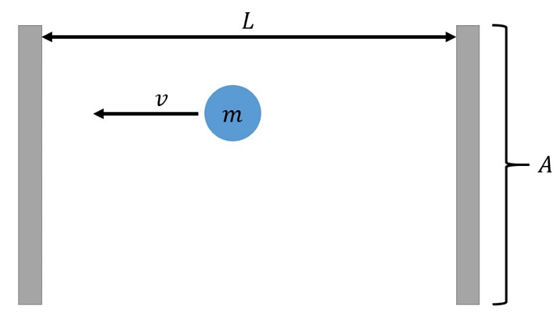
\includegraphics[width=0.7\textwidth]{2024/Abbildungen/Kinetisch_Gas/Teilchen_zwischen_Platten.png}
\end{figure}
Durch regelmäßiges Stoßen des Teilchens mit den Platten übt es einen Druck $p$ auf diese aus. 

\newpage

\enumaufgabe{\operator{Zeige}, dass der durchschnittlich auf eine Platte wirkende Druck $p$, verursacht durch Stöße mit dem einzelnen Teilchen, durch $p=\displaystyle \frac{k_\mathrm{B} T}{LA}$ gegeben ist. \\Verwende dazu das zweite \textsc{newton}sche Axiom $F=ma$, wobei $m$ die Masse, $a$ die Beschleunigung des Teilchens und $F$ die auf das Teilchen wirkende Kraft ist. Nach der kinetischen Gastheorie ist die kinetische Energie des Teilchens entlang der Bewegungsachse zwischen den Platten gegeben durch $E_{kin}=\displaystyle \frac{1}{2} k_\mathrm{B} T$.}

\solution{Kraft für Beschleunigung des Teilchens entspricht Kraft ausgewirkt auf Fläche (drittes Newtonsches Axiom) (1P)\\
Durchschnittliche Beschleunigung des Teilchens durch Aufprall auf eine Fläche:\\
$\overline{a}=\displaystyle \frac{\Delta v}{t}$ (1P) mit $\Delta v$ Geschwindigkeitsänderung beim Aufprall und $t$ Zeitabstand zwischen Zusammenstößen mit einer Fläche\\
$\Delta v=2v$(0,5 P.) und $t=\displaystyle \frac{2L}{v}$ (0,5 P.) ergibt eingesetzt:\\
$\overline{a}=\displaystyle \frac{v^2}{L}$ (1P)\\
Damit ergibt sich für die durchschnittliche Kraft nach dem zweiten Newtonschen Axiom:\\
$\overline{F} = m \frac{v^2}{L}$  (1P)\\
Mit der Definition der kinetischen Energie $E_{kin}=\displaystyle \frac{1}{2} mv^2$ folgt:\\
$\overline{F} = 2 \frac{E_{kin}}{L}$ (1P)\\
Nun kann die Beziehung $E_{kin}=\displaystyle \frac{1}{2} k_\mathrm{B} T$ verwendet werden:\\
$\overline{F} = \frac{k_\mathrm{B} T}{L}$  (1P)\\
Durch Einsetzen der durchschnittlichen Kraft in die Definition des Drucks $p=\frac{\overline{F}}{A}$ erhält man:\\
$p=\frac{k_\mathrm{B} T}{LA}$  (1P)\\
Insg. 8P
}{12cm}

\enumaufgabe{\operator{Zeige}, dass das ideale Gasgesetz $pV=nRT$ aus dem in Teilaufgabe h) hergeleiteten Ausdruck hervorgeht.\\
Hinweis: $k_\mathrm{B}=\frac{R}{N_{\mathrm{A}}}$}

\solution{
$L\cdot A$ entspricht dem Volumen eines Systems\\
Daher gilt:
$p=\displaystyle\frac{k_\mathrm{B} T}{V}$ (1P) \\
Sind nun $N$ Teilchen in diesem System vorhanden, so gilt für den Druck:\\
$p=N\displaystyle\frac{k_\mathrm{B} T}{V}$ (1P)\\
Durch Verwenden der Definition $k_\mathrm{B}=\frac{R}{N_{\mathrm{A}}}$  für die Boltzmann-Konstante erhält man:\\
$p=\displaystyle\frac{N RT}{N_{\mathrm{A}} V}$ (1P)\\
$N/N_{\mathrm{A}}$ entspricht dabei der Stoffmenge n, womit man das ideale Gasgesetz erhält:\\
$pV=nRT$ (1P)\\
Insg. 4P
}{6cm}
\solutiontext{$\sum$ 34 P.}{}
\end{document}